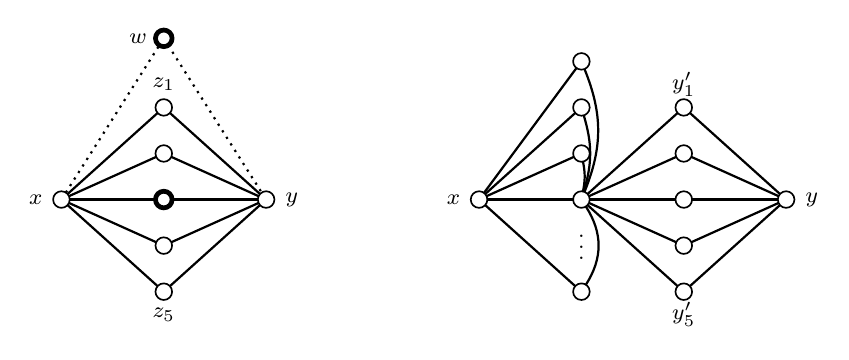
\begin{tikzpicture}[thick, scale=.65, yscale=.9]
  % node styles
  \tikzstyle{uStyle}=[circle, minimum size=6pt, inner sep=0pt, outer sep=0pt, draw, fill=white, semithick]
  \tikzstyle{sStyle}=[rectangle, minimum size=4.5pt, inner sep=0pt, outer sep=0pt, draw, fill=white, semithick]
  \tikzstyle{lStyle}=[circle, minimum size=4.5pt, inner sep=0pt, outer sep=0pt, draw=none, fill=none]
  \tikzset{every node/.style=uStyle}
  \def\off{.5cm}

  %---------------- Left figure ----------------
  % five Z-vertices
  \foreach \i in {1,...,5}
    \draw (0,3-\i) node (z\i) {};

  % terminals x and y
  \draw (-2,0) node (x) {} (2,0) node (y) {};

  % complete bipartite connections K_{2,5}
  \foreach \i in {1,...,5}
    \draw (x) -- (z\i) -- (y);

  % labels
  \draw (x) ++ (-\off,0) node[lStyle] {\footnotesize{$x$}};
  \draw (y) ++ ( \off,0) node[lStyle] {\footnotesize{$y$}};
  \draw (z1) ++ (0,\off) node[lStyle] {\footnotesize{$z_1$}};
  \draw (z5) ++ (0,-\off) node[lStyle] {\footnotesize{$z_5$}};

  % emphasize w and z3
  \draw (0,3.5) node[line width=.6mm] (w) {} ++ (-\off,0) node[lStyle] {\footnotesize{$w$}};
  \draw (z3) node[line width=.6mm] {};

  % dotted apex connections
  \draw[dotted] (x) -- (w) -- (y);

  %---------------- Right figure ----------------
  \begin{scope}[xshift=4in]
    % five Y-vertices
    \foreach \i in {1,...,5}
      \draw (0,3-\i) node (y\i) {};

    % path x -- x4 -- y
    \draw (-4,0) node (x) {} -- (-2,0) node (x4) {} (2,0) node (y) {};

    % connections from x4 to Y and from Y to y
    \foreach \i in {1,...,5}
      \draw (x4) -- (y\i) -- (y);

    % neighbors of x on the left column (x1, x2, x3, x6)
    \foreach \i in {1,2,3,6}
      \draw (-2,4-\i) node (x\i) {} -- (x);

    % curved edges from x4 to these x_i
    \draw (x4) edge[bend right=20] (x1);
    \draw (x4) edge[bend right=15] (x2);
    \draw (x4) edge[bend right=10] (x3);
    \draw (-2,-.85) node[lStyle] {\footnotesize{$\vdots$}};
    \draw (x4) edge[bend left] (x6);

    % labels
    \draw (x) ++ (-\off,0) node[lStyle] {\footnotesize{$x$}};
    \draw (y) ++ ( \off,0) node[lStyle] {\footnotesize{$y$}};
    \draw (y1) ++ (0,\off) node[lStyle] {\footnotesize{$y'_1$}};
    \draw (y5) ++ (0,-\off) node[lStyle] {\footnotesize{$y'_5$}};
  \end{scope}
\end{tikzpicture}